%
\documentclass{article}
\usepackage{hyperref}
\usepackage[english]{babel}
\usepackage{Sweave}
\begin{document}

\Sconcordance{concordance:Week1.tex:Week1.Rnw:%
1 4 1 1 0 47 1 1 4 1 3 5 0 1 2 2 1 1 2 1 0 1 1 6 0 1 2 2 1 1 3 2 0 1 2 %
1 0 1 2 6 0 1 2 3 1 1 2 1 0 1 5 8 0 1 4 6 0 1 2 5 1 1 10 4 0 3 1 3 0 1 %
2 5 1 1 2 8 0 1 2 2 1 1 2 7 0 1 2 3 1 1 2 1 0 1 1 6 0 1 2 2 1 1 2 12 0 %
1 1 6 0 1 2 4 1 1 7 10 0 1 2 8 1 1 6 9 0 1 2 2 1 1 2 1 0 1 1 6 0 1 2 2 %
1 1 2 7 0 1 2 3 1 1 4 7 0 1 2 7 1 1 2 7 0 1 2 3 1 1 2 13 0 1 2 5 1 1 2 %
1 0 1 1 6 0 1 2 7 0 1 2 3 1 1 2 6 0 1 1 6 0 1 2 4 1 1 2 1 0 1 1 6 0 1 2 %
2 1 1 2 7 0 1 2 3 1 1 2 7 0 1 2 1 1 1 3 8 0 1 2 5 1}


\title{Problem Set 1}
\author{\href{http://feliperiveroll.name}{Felipe Riveroll Aguirre}\footnote{\texttt{friveroll@gmail.com}}} 
\maketitle

\textbf{Types of Data.} Decide if the following are examples of discrete or continuous data

\begin{enumerate}
  \item The number of deaths in the United States in a specific year\\
\textbf{a) Discrete}, b) Continuous\\ 
  \item The concentration of chlorine in a sample of water\\
a) Discrete, \textbf{b) Continuous}\\ 
  \item The length of time to recovery after a heart attack\\
a) Discrete, \textbf{b) Continuous}\\ 
  \item The number of adults hospitalized for respiratory disease during the summer of 2009 in Beijing\\
\textbf{a) Discrete}, b) Continuous \\
\end{enumerate}

\pagebreak

\textbf{Frequency.} In this question, we examine the reported numbers of hospitalizations for cardiac events in the United States for each month in the period January 1991 to December 1992.

\begin{table}[ht]
\begin{center}
\begin{tabular}{cccc}
  \hline
Month 1991 & Number 1991 & Month 1992 & Number 1992 \\ 
  \hline
January & 325 & January & 317 \\ 
February & 312 & February & 302 \\ 
March & 346 & March & 339 \\ 
April & 340 & April & 328 \\ 
May & 355 &   May & 361 \\ 
June & 342 &   June & 333 \\ 
July & 358 &   July & 341 \\ 
August & 346 &   August & 343 \\ 
September & 365 &   September & 359 \\ 
October & 355 &  October & 305 \\ 
November & 324 &  November & 312 \\ 
December & 342 &  December & 321 \\ 
   \hline
\end{tabular}
\end{center}
\end{table}


\begin{Schunk}
\begin{Sinput}
> hospitalizations <- 
+   read.csv("https://dl.dropbox.com/u/4828275/hospitalizations.csv")
\end{Sinput}
\end{Schunk}

\begin{enumerate}
  \item In the year 1991, what is the relative frequency of hospitalizations in September?
\begin{Schunk}
\begin{Sinput}
> sep1991.rf <- hospitalizations[9,2]/sum(hospitalizations[2])
> print(sep1991.rf)
\end{Sinput}
\begin{Soutput}
[1] 0.08880779
\end{Soutput}
\end{Schunk}

  \item Is the absolute frequency of hospitalizations in September 1991 greater than the absolute frequency of hospitalizations in September 1992?

\begin{Schunk}
\begin{Sinput}
> sep1991.af <- hospitalizations[9,2]/
+   (sum(hospitalizations[2])+ sum(hospitalizations[4]))
> sep1992.af <- hospitalizations[9,4]/
+   (sum(hospitalizations[2])+ sum(hospitalizations[4]))
> sep1991.af > sep1992.af
\end{Sinput}
\begin{Soutput}
[1] TRUE
\end{Soutput}
\end{Schunk}
\pagebreak
  \item Restricting to the year 1992, calculate the relative frequency of hospitalizations in September.  Comparing this estimate with the relative frequency calculation in part (a), is the relative frequency of hospitalizations in September higher in 1991 or in 1992?
  
  
\begin{Schunk}
\begin{Sinput}
> sep1992.rf <- hospitalizations[9,4]/sum(hospitalizations[4])
> if (sep1991.rf < sep1992.rf)
+ {
+   print("1992")
+ }
\end{Sinput}
\begin{Soutput}
[1] "1992"
\end{Soutput}
\begin{Sinput}
> if (sep1991.rf > sep1992.rf)
+ {
+   print("1991")
+ }
\end{Sinput}
\end{Schunk}


\end{enumerate}
\pagebreak

\textbf{Prevalent hypertension}. In this question, we use data from the NHLBI teaching data set.  Our study population is the 4,434 participants in the Framingham Heart Study attending the first examination in 1956.   Using the Framingham dataset, we explore data types, tables, and graphs in this question.  We will examine the indicator of prevalent hypertension at exam 1 in 1956 (variable name: prevhyp1).  
\begin{Schunk}
\begin{Sinput}
> if (!"foreign" %in% installed.packages())
+ {
+   install.packages("foreign", dependencies = TRUE)
+ }
> library("foreign") 
> data <- read.dta("https://dl.dropbox.com/u/4828275/fhs.dta")
> attach(data)
\end{Sinput}
\end{Schunk}

\begin{enumerate}
  \item Prevalent hypertension at exam 1 is an example of what type of data?\\
(a) nominal, (b) binary, \textbf{(c) both a and b}
  \item How many individuals in the study population had prevalent hypertension at exam 1?
  
\begin{Schunk}
\begin{Sinput}
> summary(prevhyp1)[2]
\end{Sinput}
\begin{Soutput}
 Yes 
1430 
\end{Soutput}
\end{Schunk}

  \item What is the relative frequency of prevalent hypertension at exam 1?

\begin{Schunk}
\begin{Sinput}
> as.vector(summary(prevhyp1)[2])/length(prevhyp1)
\end{Sinput}
\begin{Soutput}
[1] 0.3225079
\end{Soutput}
\end{Schunk}


\item Among the individuals with prevalent hypertension at exam 1, how many are female?

\begin{Schunk}
\begin{Sinput}
> prevhyp1_fem <- length(prevhyp1[prevhyp1 == "Yes" & sex1 == "Female"])
> print(prevhyp1_fem)
\end{Sinput}
\begin{Soutput}
[1] 799
\end{Soutput}
\end{Schunk}
\pagebreak
  \item What proportion of individuals with prevalent hypertension at exam 1 are female? Express your answer as a proportion of the whole (e.g. 10\% would be .10).

\begin{Schunk}
\begin{Sinput}
> by(prevhyp1, sex1, summary)
\end{Sinput}
\begin{Soutput}
sex1: Male
  No  Yes 
1313  631 
------------------------------------------------------------ 
sex1: Female
  No  Yes 
1691  799 
\end{Soutput}
\begin{Sinput}
> prevhyp1_fem/length(prevhyp1[prevhyp1 == "Yes"])
\end{Sinput}
\begin{Soutput}
[1] 0.5587413
\end{Soutput}
\end{Schunk}


\item Which graph would you use to summarize the distribution of the indicator for prevalent hypertension at exam 1 in the study population?\\
(a) scatter plot, (b) histogram, \textbf{(c) bar chart}

\begin{Schunk}
\begin{Sinput}
> barplot(table(prevhyp1, sex1)[c(2,4)], 
+         col=c("darkblue","red"), 
+         ylim=c(0,800), 
+         names.arg=c("Male", "Female"), 
+         xlab="Sex", 
+         ylab="Prevalent hypertension at exam 1")
\end{Sinput}
\end{Schunk}
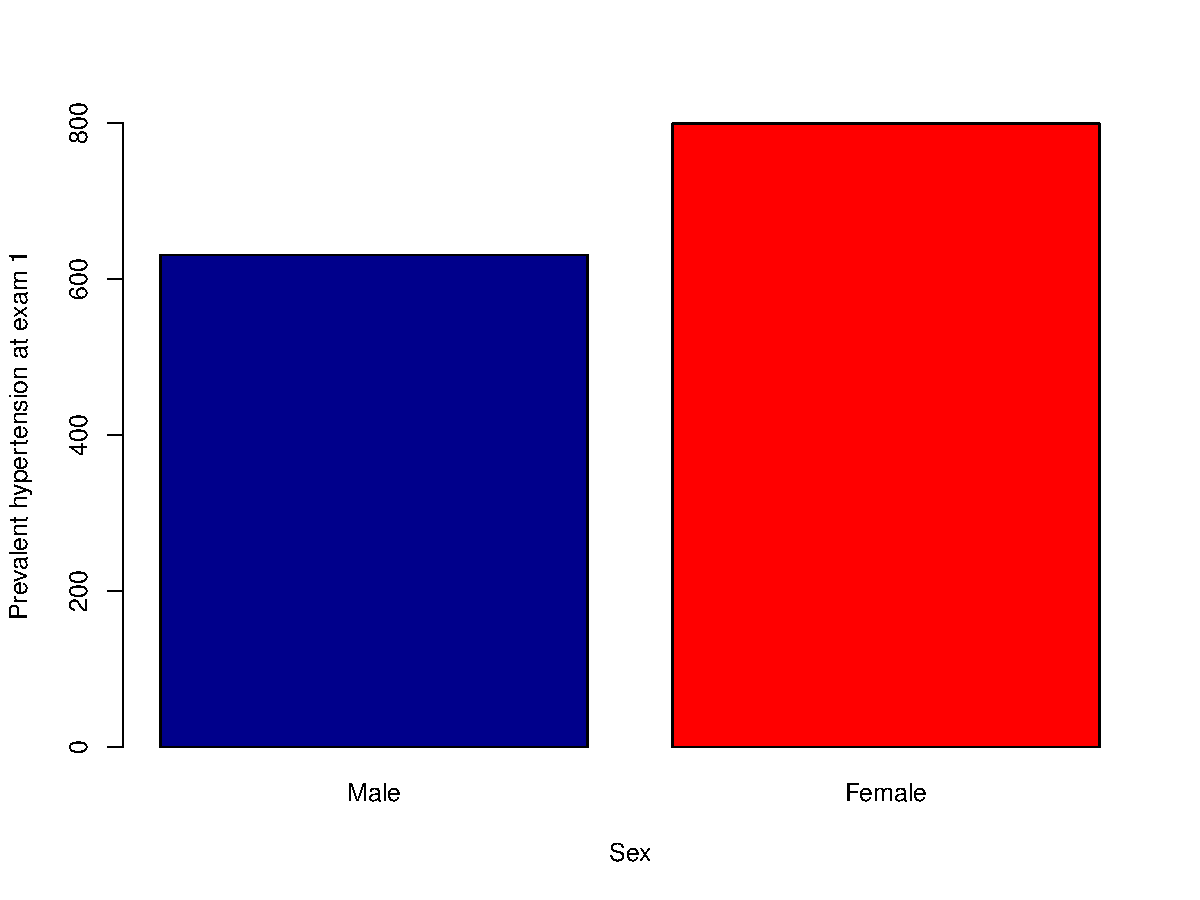
\includegraphics{Week1-barchart}
\end{enumerate}
\pagebreak

\textbf{BMI at baseline.} In this question, we again use data from the NHLBI teaching data set to examine the continuous variable, body mass index (BMI). Our study population is the subset of participants in the Framingham Heart Study attending the first examination in 1956 with a nonmissing BMI measure (4,415 participants out of 4,434).  

\begin{enumerate}
  \item To quickly examine the interquartile range for BMI at exam 1 in the study population, which graph would you use?\\
(a) histogram, \textbf{(b) boxplot}, (c) scatter plot

\begin{Schunk}
\begin{Sinput}
> boxplot(bmi1~sex1, 
+         xlab="Sex", 
+         ylab="BMI", 
+         main="Body Mass Index at exam 1", 
+         col=c("darkblue","red"))
\end{Sinput}
\end{Schunk}
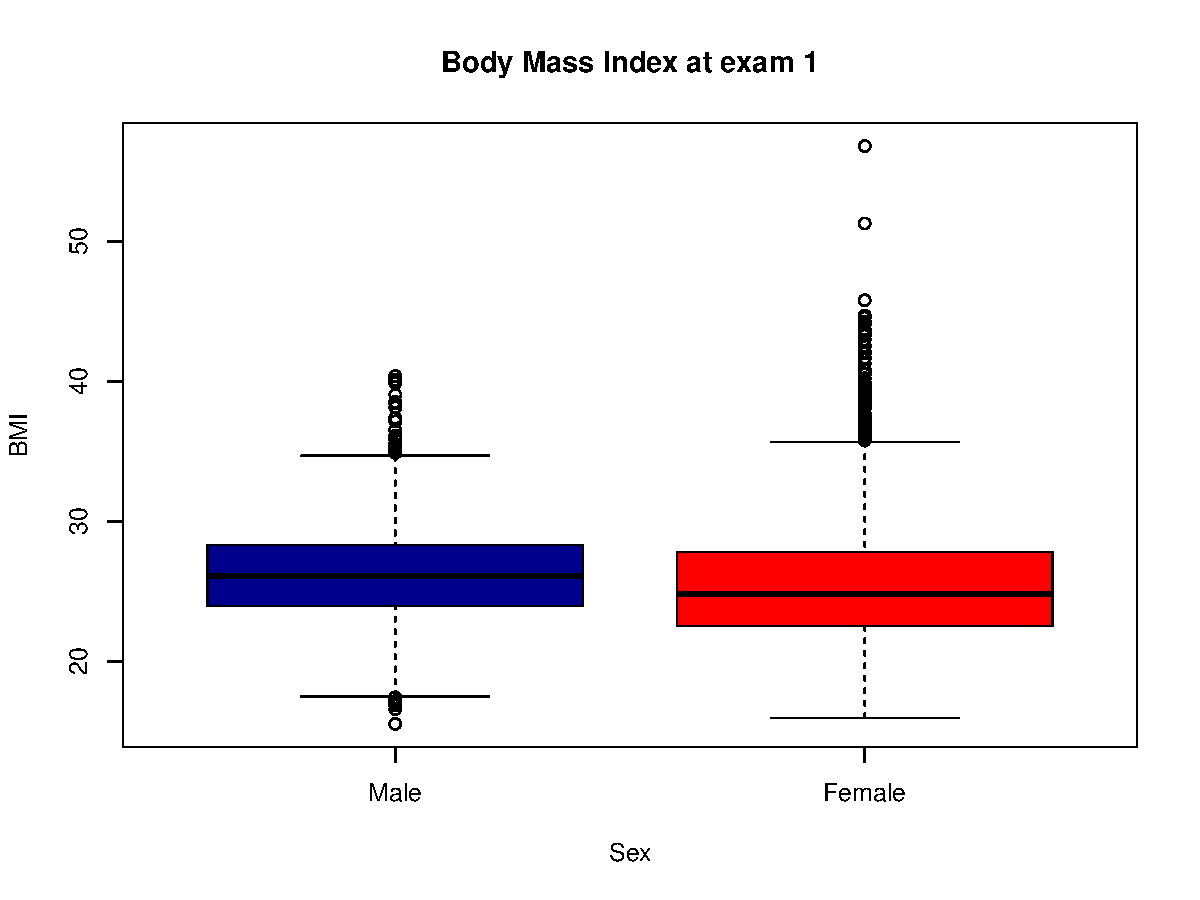
\includegraphics{Week1-boxplot}

\item We say an individual has high BMI at exam 1 if his BMI is greater than 25.  How many individuals in the dataset have high BMI at exam 1?  

\begin{Schunk}
\begin{Sinput}
> high_bmi1 <- length(na.omit(bmi1[bmi1>25]))
> print(high_bmi1)
\end{Sinput}
\begin{Soutput}
[1] 2422
\end{Soutput}
\end{Schunk}
\pagebreak
\item Out of the 4,415 participants with a BMI measurement at exam 1. What percent had high BMI at exam 1) (an individual has high BMI at exam 1 if his BMI is greater than 25) Express your answer as a proportion of the whole (e.g. 10\% would be .10).

\begin{Schunk}
\begin{Sinput}
> high_bmi1/length(na.omit(bmi1))
\end{Sinput}
\begin{Soutput}
[1] 0.5485844
\end{Soutput}
\end{Schunk}

Restricting to the population with BMI measurements at both exam 1 and exam 2, make a scatter plot of BMI at exam 1 (bmi1) versus BMI at exam 2 (bmi2). In general,higher BMI at exam 1 is associated with a  \_\_\_\_\_\_\_\_\_  BMI at exam 2.\\
\textbf{(a) higher}, (b) lower

\begin{Schunk}
\begin{Sinput}
> plot(bmi1~bmi2, 
+      main="Body Mass Index at exam 1 Vs. 2",
+      col=c("darkblue","red"))
\end{Sinput}
\end{Schunk}
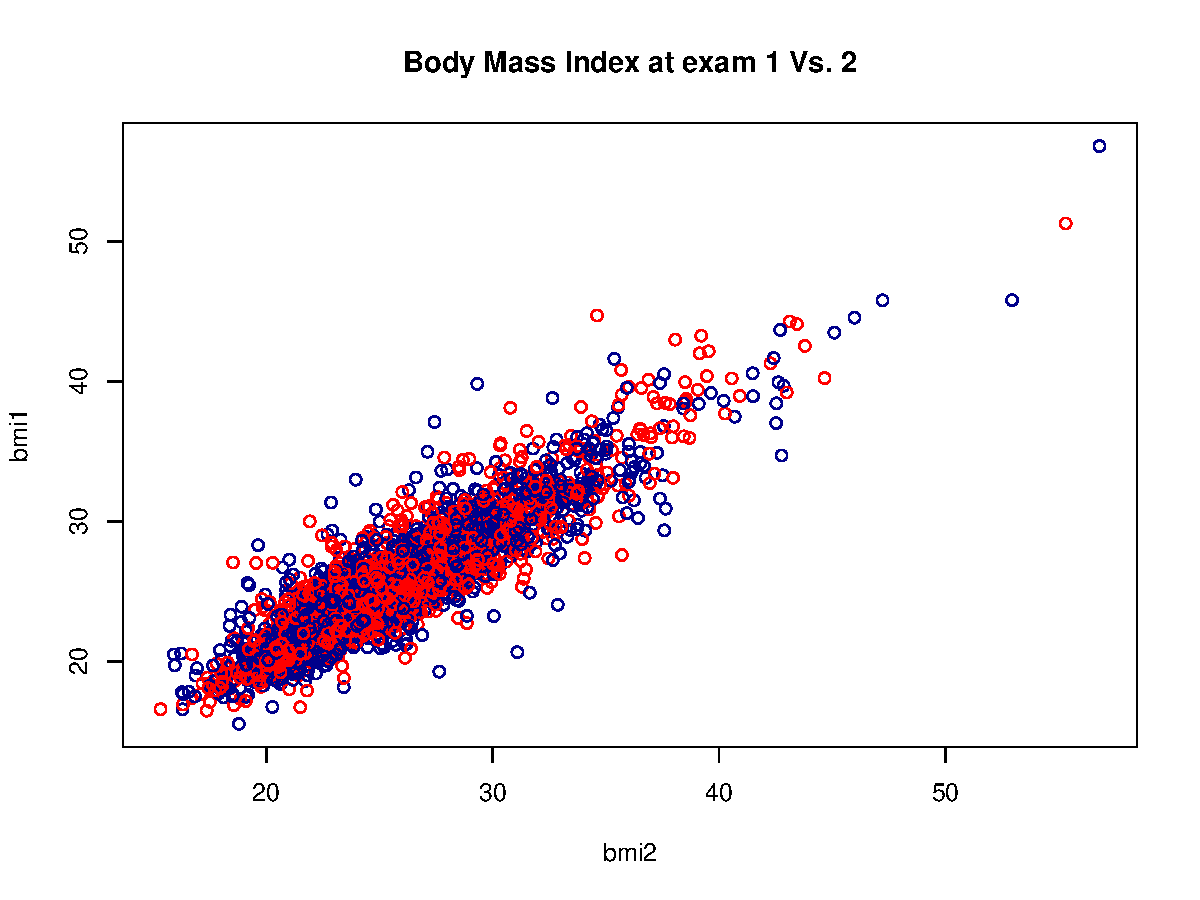
\includegraphics{Week1-scatter}

\end{enumerate}
\pagebreak
\textbf{BMI over time.} In this question, we again use data from the NHLBI teaching data set to examine the continuous variable, body mass index (BMI).   Our study population is the subset of participants in the Framingham Heart Study attending the first examination in 1956 with a nonmissing BMI measure (4,415 participants out of 4,434). 

\begin{enumerate}
  \item What is the mean BMI at exam 1 in the study population?

\begin{Schunk}
\begin{Sinput}
> mean(bmi1, na.rm=T)
\end{Sinput}
\begin{Soutput}
[1] 25.84616
\end{Soutput}
\end{Schunk}

\item The median BMI at exam 1 is 25.45 in the study population.  Comparing the mean and median, do these data suggest that the distribution of BMI at exam 1 is right skewed or left skewed?\\
\textbf{(a) right skewed},  (b) left skewed

\begin{Schunk}
\begin{Sinput}
> by(bmi1, sex1, summary)
\end{Sinput}
\begin{Soutput}
sex1: Male
   Min. 1st Qu.  Median    Mean 3rd Qu.    Max.    NA's 
  15.54   23.97   26.08   26.17   28.32   40.38       5 
------------------------------------------------------------ 
sex1: Female
   Min. 1st Qu.  Median    Mean 3rd Qu.    Max.    NA's 
  15.96   22.54   24.83   25.59   27.82   56.80      14 
\end{Soutput}
\end{Schunk}

\item Is the mean BMI at exam 1 higher in males or females?\\
\textbf{(a) Males},  (b) Females

\item Should you compare the mode for BMI at exam 1 in males versus females?\\
(a) Yes, \textbf{(b) No}
\begin{Schunk}
\begin{Sinput}
> bmi1_by_sex1 <- table(bmi1, sex1) 
> subset(bmi1_by_sex1[,1], bmi1_by_sex1[,1]==max(bmi1_by_sex1[,1])) 
\end{Sinput}
\begin{Soutput}
26.09 
   11 
\end{Soutput}
\begin{Sinput}
> subset(bmi1_by_sex1[,2], bmi1_by_sex1[,2]==max(bmi1_by_sex1[,2]))
\end{Sinput}
\begin{Soutput}
22.19 22.91 23.48 
   17    17    17 
\end{Soutput}
\end{Schunk}
\pagebreak
\item Is the IQR for BMI at exam 1 larger in males or females?\\
(a) Males, \textbf{(b) Females}

\begin{Schunk}
\begin{Sinput}
> IQR(bmi1[sex1=="Female"], na.rm=T) 
\end{Sinput}
\begin{Soutput}
[1] 5.28
\end{Soutput}
\begin{Sinput}
> IQR(bmi1[sex1=="Male"], na.rm=T)
\end{Sinput}
\begin{Soutput}
[1] 4.35
\end{Soutput}
\end{Schunk}
\pagebreak
\textbf{Now, for the remaining parts of this question, restrict your study population to the subset of participants with BMI measures at exam 1 and exam 2.  }

\item What is the mean change in BMI from exam 1 to exam 2? Change in BMI is defined as BMI at exam 2 minus BMI at exam1. (Note: you need to generate this variable in R).

\begin{Schunk}
\begin{Sinput}
> bmi_delta_12 <- na.omit(bmi2 - bmi1)
> mean(bmi_delta_12)
\end{Sinput}
\begin{Soutput}
[1] 0.06783065
\end{Soutput}
\end{Schunk}

\item What is the standard deviation of the change in BMI from exam 1 to exam 2?

\begin{Schunk}
\begin{Sinput}
> sd(bmi_delta_12)
\end{Sinput}
\begin{Soutput}
[1] 1.801516
\end{Soutput}
\end{Schunk}


\item What is the range of changes in BMI from exam 1 to exam 2?

\begin{Schunk}
\begin{Sinput}
> max(bmi_delta_12) - min(bmi_delta_12)
\end{Sinput}
\begin{Soutput}
[1] 20.93
\end{Soutput}
\end{Schunk}

\item Assuming that the empirical rule applies in this situation, we expect that 95\% of individuals will have a change in BMI between exams 1 and 2 that lies within the interval 
\begin{Schunk}
\begin{Sinput}
> c(mean(bmi_delta_12)-2*sd(bmi_delta_12), 
+   mean(bmi_delta_12)+2*sd(bmi_delta_12))
\end{Sinput}
\begin{Soutput}
[1] -3.535202  3.670864
\end{Soutput}
\end{Schunk}
\end{enumerate}

\item Does it appear that the empirical rule can be used in the previous question, examining the change in BMI from exam 1 to exam 2?\\
\textbf{(a) Yes}, (b) No

\end{document}
